\chapter{Data Extraction and Preprocessing} 
\label{Chapter3}

This chapter details the data sources used to train the various credit scoring models developed throughout this project, the various data extraction techniques used to extract the alternative data features within the training sets, and the pre-processing and feature engineering techniques deployed before the modelling phase.   
%---------------------------------------------------------------------------------------
%	SECTION 1
%---------------------------------------------------------------------------------------

\section{Data Used}

\subsection{Providers}

There were two main sources that provider the data used to train the models developed throughout this project. \\

The first data provider is a Nigerian micro-finance institution that has disbursed loans to more than 250,000 consumers. The institution is an application-based lender and currently only provides credit to android users. The institution, with its customers' consent, gains access to the data on customers' devices. This data includes SMS data, contact data and location data. On top of the alternative data collected, sociodemographic data is collected via customer input on the institution's application. \\

The second source of data for this project was the Nigerian credit bureaus CRC, CRS and XDS. It is mandatory for credit providing institutions in Nigeria to submit their customers' credit performance data to these credit bureaus.

\subsection{Personal Data}

It is key to note that no personal data, data that relates to an identified or could be used to identify a living individual, was not made publicly available, used within the creation of features, or used to train the models developed throughout this project. 

\subsection{Dataset}

A final dataset was created for first time loan customers of the micro-finance institution that had existing credit bureau data prior to their first application. The customers required existing credit data as it was needed in order to compare the performance of first time credit credit scoring models that use only alternative data or alternative data in conjunction with sociodemographic data, against first time credit scoring models that make use of existing credit data. The final dataset consisted of 49,550 customers/loans. 

\subsection{Data Categories}

Three major data categories were drawn from the data sources. These categories were sociodemographic data, credit bureau data and alternative data. The main aim of this thesis is to assess how alternative data can augment traditional credit scoring data. To complete this aim various combinations of these data categories were used to develop various credit scoring models. The statistical performance of the models were assessed in order to test whether using the various data categories resulted in a significant difference in model performance. 

%---------------------------------------------------------------------------------------
%	SECTION 2
%---------------------------------------------------------------------------------------

\section{Data Extraction and Feature Engineering}

\subsection{Sociodemographic and Credit Bureau Data}

The more traditional credit scoring features, developed from sociodemographic and credit bureau data attached to each first-time borrower, were created and extracted using SQL (Structured Query Language). The data was extracted from the company's relational database. \\

The query was written in a manner that ensured that no data leakage would occur when the credit scoring models were being trained. This means that only data that would be known at the point in time when a particular client applied for their loan could be sued to develop features. The only case were data was used that would not be known at the point in time of application was repayment data, as this was used to develop the default (whether the client repaid their loan or not) target variable. \\

The overall query used to extract the sociodemographic and credit bureau for each loan was a collection of sub-queries joined on a unique key attached to each loan. The query used to extract the credit bureau required an aggregation in order to generate features that represented the total number of loans each client had prior to their application with the micro-finance institution used in this study. The credit bureau features used in the modelling process and their definitions can be found in the appendix of this paper. The sociodemographic data was extracted using a simpler sub-query,  like the credit bureau features their definitions can be found in the appendix of this paper.  \\


\subsection{Alternative Data}

The three main sources of alternative data used to develop features were the application, SMS, and device data stored on each customers' cellphone. The data was extracted from the micro-finance institution's using PyMongo, a Python package that allows a user to query data from a Mongo database from within a Python script. The application and SMS data was extracted from different Mongo databases, however expressions (regex) were used to filter both data types and to develop features. Regex functions are sets of sequences of characters that define a particularly search pattern. The functions are then used to identify cases of the defined pattern in strings \parencite{Regex}. \\

The device data was extracted from a separate database as the application and SMS data and an entirely different technique was used to generate features from the data. The technique used in this case was web scraping, which is a method of extracting data from websites \parencite{WebScraping}. 

\subsubsection{Application Based Features}

The application based features engineered for this project were counts of particular applications present on a clients device at the point in time of their application. The features included a count of the finical, competing micro-finance, news, gambling and virtual private network (VPN) applications. The counts were generated by first compiling a list of all unique applications on a client's. Then the name of each application was passed through a series of regular expression key word searches. Each expression was designed to detect a specific application type. If  a particular application type search resulted in a match, the count associated with that search was updated. \\

The process developed to pass an application through the application extracting regular expressions and how the count features were generated throughout this process is represented in Figure \ref{fig:app_features}. The process was coming up completed for every unique application recorded on the client's device. 


\vspace{10 pt}

\begin{figure}[!htb]
\centering
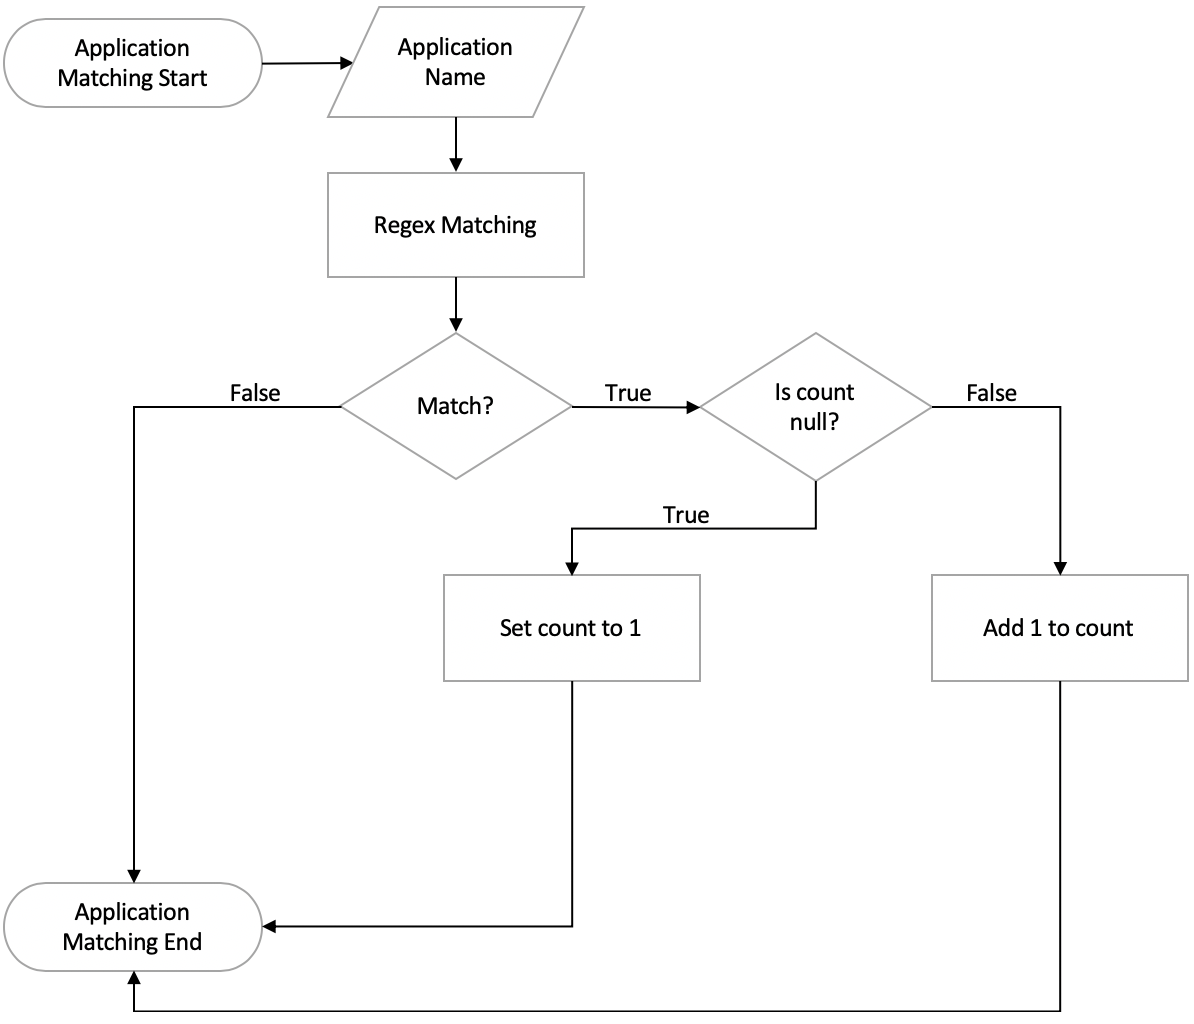
\includegraphics[width=0.55\textwidth]{images/app_feats.png}
\caption{Application Based Feature Generation}
\label{fig:app_features}
\end{figure}


\subsubsection{SMS Based Features}

The SMS data consisted of messages received by the clients in the 90 days prior to their application, by nature this data is more sensitive than the other data used throughout this research. Similarly to the process developed to generate the application based features, each message received by a client was complied into a list. The list was the looped over in order to generate features for each client. \\

In order to avoid exposing personal messages the each message was passed through two filtering regular expressions. The first expression returned only messages received from Nigerian banks, while the second ensured that only messages returned by competitor micro-finance institutions were returned. The regular expressions had a dual purpose. They prevented exposure to sensitive content and they acted as the first step in the SMS based feature generation process. \\

If a message passed through the regular expression for banking messages it was exposed to the banking feature creation process. Typically, messages from Nigerian banks have a similar structure. They display a transaction amount, the date of the transaction, the type of transaction (credit or debit to the account), and finally the balance in the account after the transaction. Regular expressions were used these features and store them as either numeric variables or lists.  \\

If a message did not pass through the banking regular expression it was then passed to the competitor expression. If the message passed through this expression it was then further screened by another set of regex functions. These functions searched for key words in order to identify if a client had another loan with a competitor and if that loan had been repaid successfully or not. The actual loan amount was extracted using regex as was the loan repayment (instalment amount). These amounts were appended to lists. \\

After the passing every message associated to a particular client through the regex functions the lists created throughout the process were used to generate the SMS based features for that particular client. \\

\vspace{10pt}

The banking related features generated were:

\begin{itemize}
    \item The number of unique banks that sent the client a message
    \item The minimum and maximum debit transaction, credit transaction and account balance values extracted
    \item The total number of debit and credit transactions recorded
    \item The number of times the term 'insufficient funds' was recorded in the client's messages
\end{itemize}

\vspace{10pt}

The process of passing an SMS through the bank related regular expressions and how the banking features were generated throughout that process is represented in Figure \ref{fig:bank_features}. The process was completed for every message received by a client within the 90 day period prior to their application. 

\vspace{10pt}

\begin{figure}[!htb]
\centering
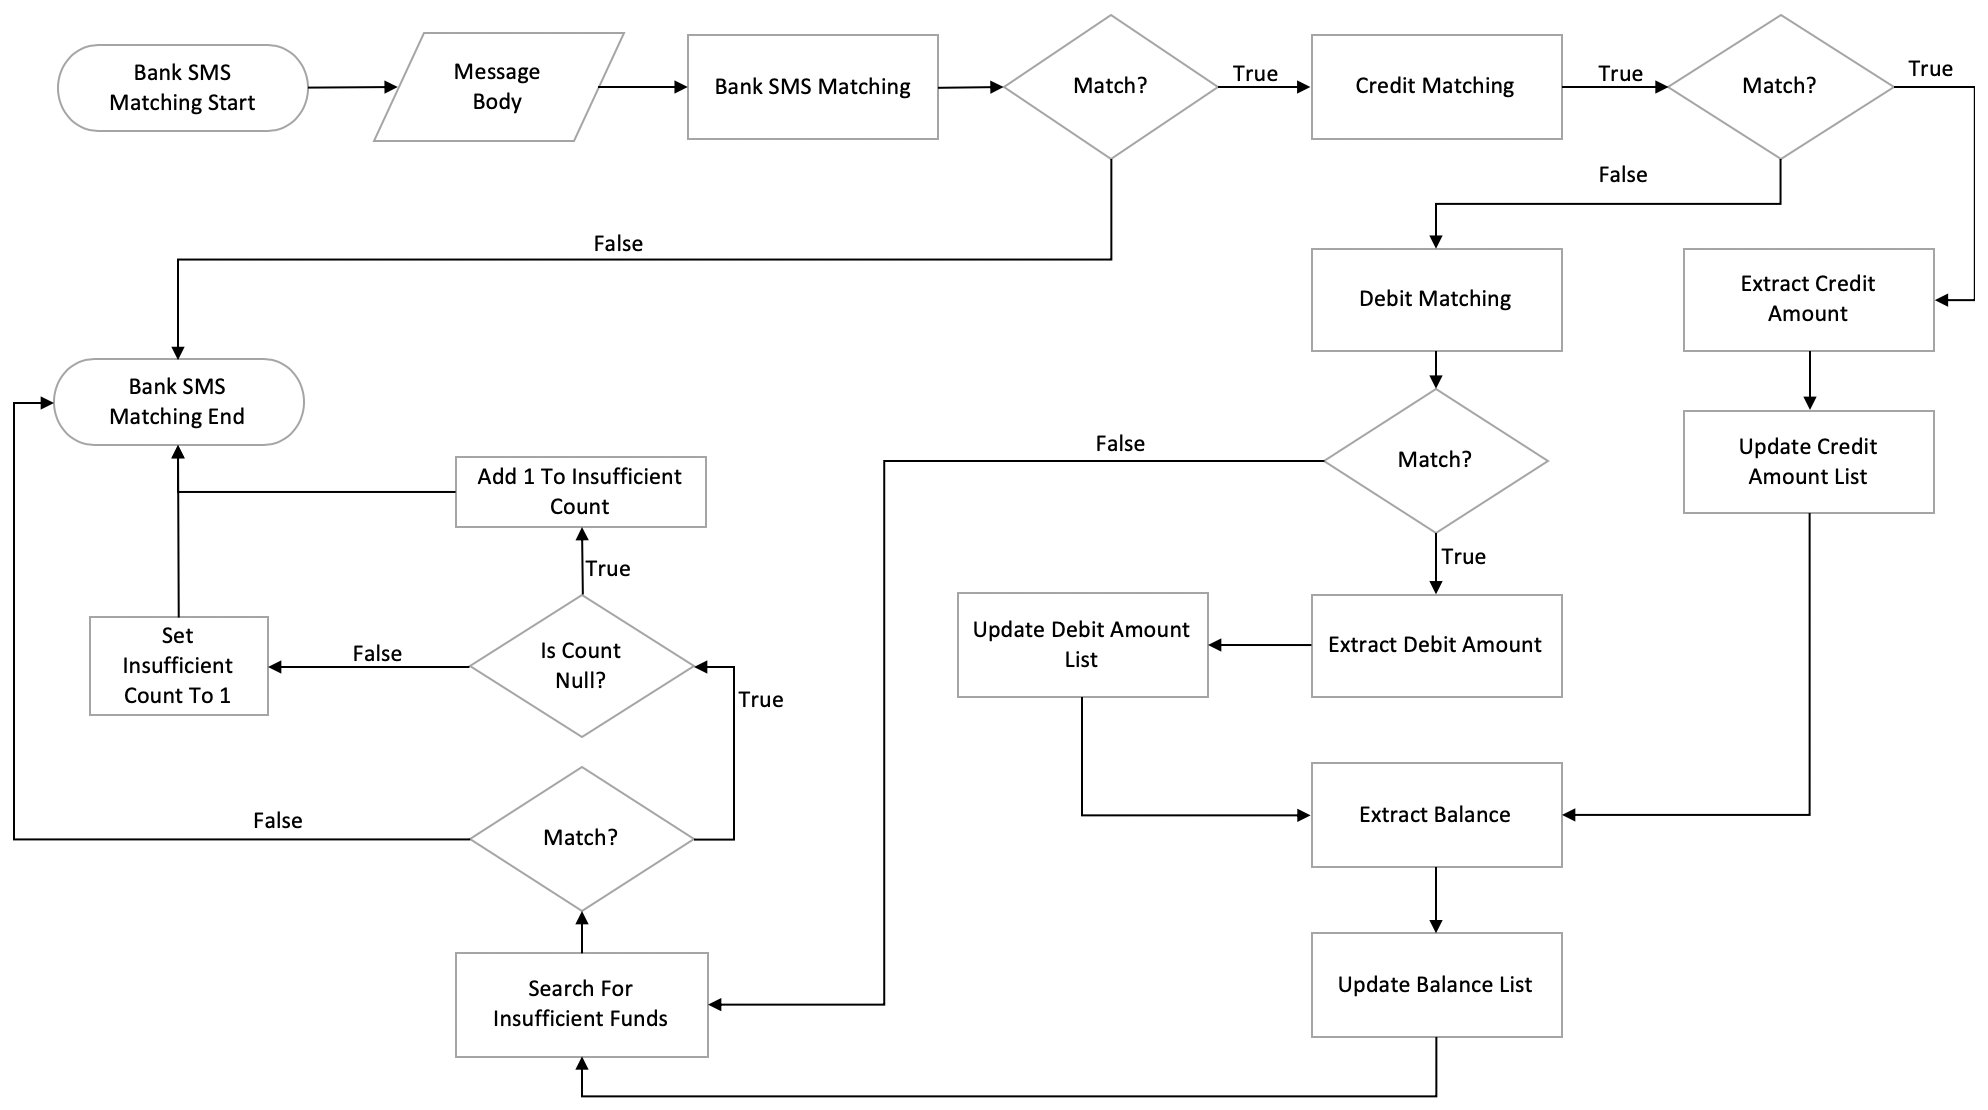
\includegraphics[width=0.9\textwidth]{images/bank_feats.png}
\caption{Bank Based Feature Generation}
\label{fig:bank_features}
\end{figure}

\vspace{10pt}

\newpage

The competitor related features generated were:

\begin{itemize}
    \item The number of competitors that sent the client a message
    \item The number of competitors that sent a loan to the client
    \item The minimum and maximum loan amount received by, successful loan repayment made by, and unsuccessful loan repayment made by the client
    \item The number of loans received by, successful loan repayments made by, and unsuccessful loan repayments made by the client
    \item The number of rejected loan applications made by the client. 
\end{itemize}

\vspace{10pt}

The process of passing an SMS through the competitor related regular expressions and how features were generated throughout that process is represented in Figure \ref{fig:comp_features}. The process was completed for every SMS message received by a client within the 90 day period prior to their application. 

\vspace{10pt}

\begin{figure}[!htb]
\centering
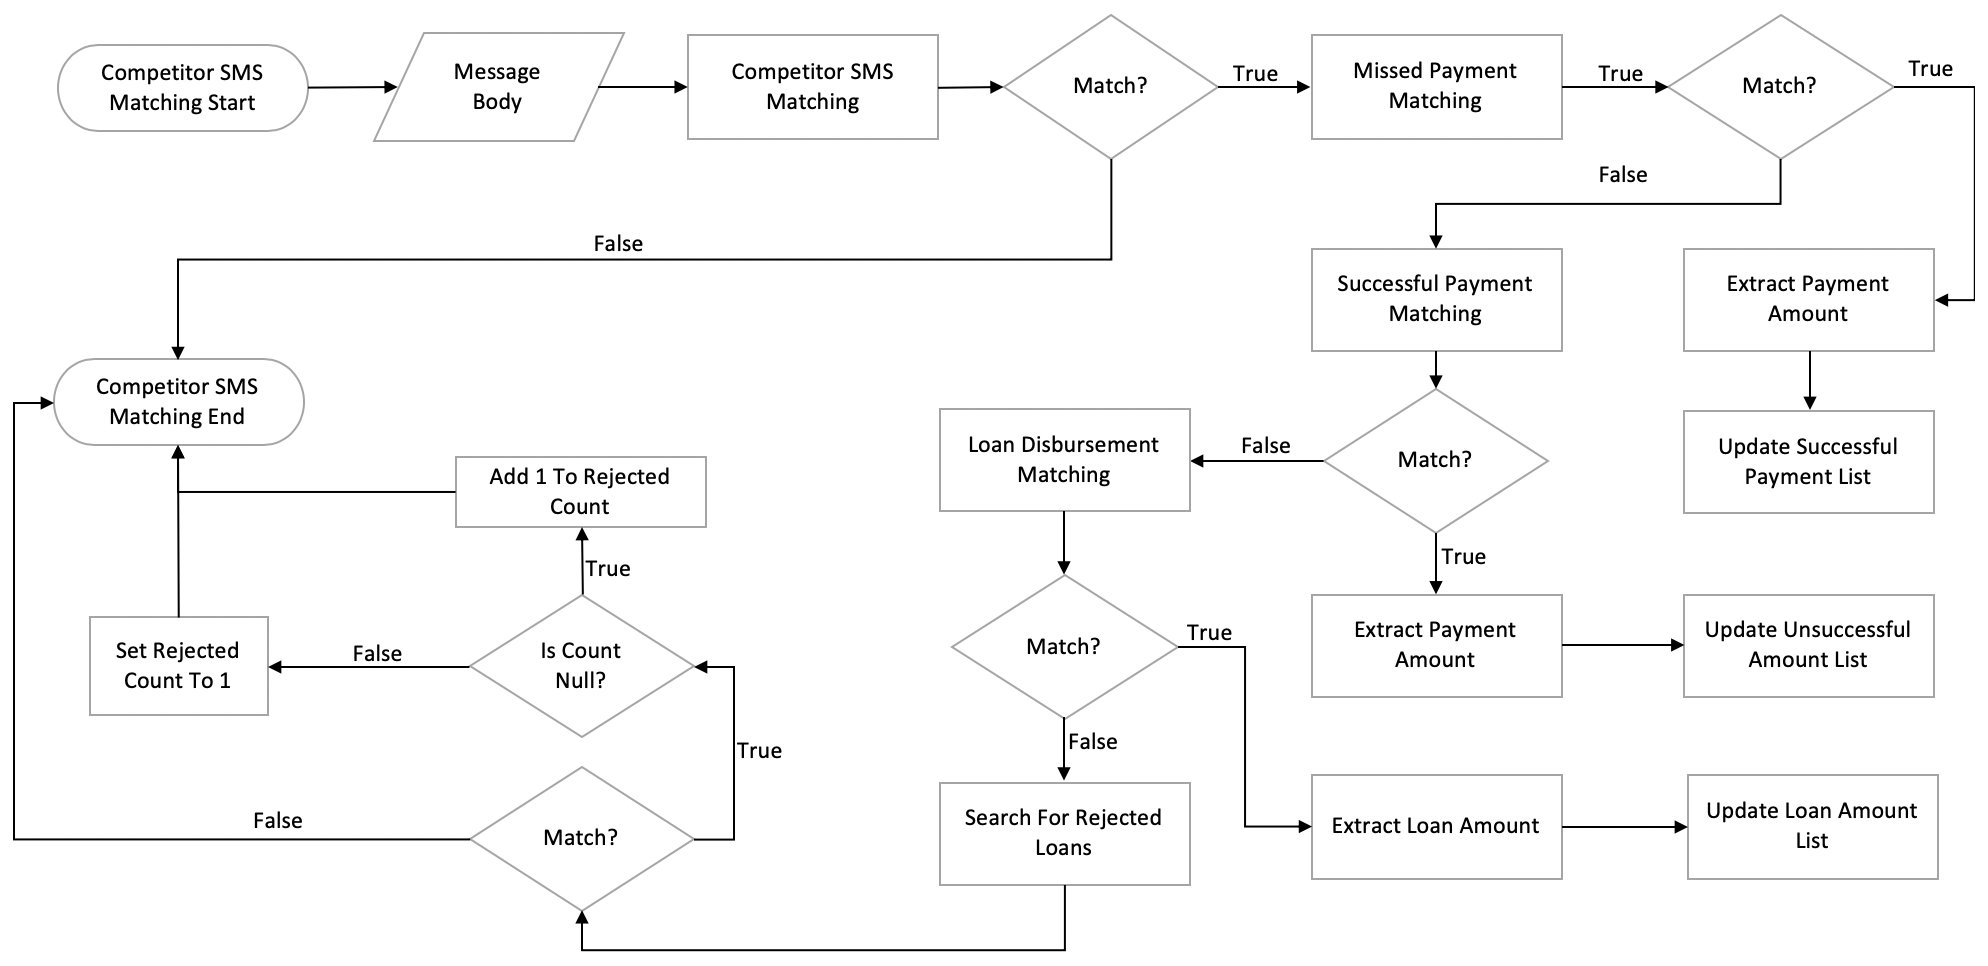
\includegraphics[width=0.95\textwidth]{images/comp_feats.png}
\caption{Competitor Based Feature Generation}
\label{fig:comp_features}
\end{figure}

\vspace{10pt}


\subsubsection{Web Scraping}

The unique Android ID attached to each customer's cellular device, used to apply for their loan, was used to ascertain the brand and model of the device as well as the operating version currently used on the device. The brand of device and operating system system were used directly as features while the device brand name and model were used in conjunction to scrape the price of the device. \\

The script written to scrape and calculate the device price was written in Python and made use of the Beautiful Soup web scraping package. The price of each device was scraped from Jumia and Kara, two of the biggest Nigerian e-commerce platforms. \\

The price was scraped from both websites by passing the name and model of the device into the respective search URL of each website. The Jumia search URL appears as follows \url{https://www.jumia.com.ng/phones-tablets/?q={NameAndBrand}&sort=Price}. The price was then scraped from the first page returned by the search. The prices were contained within specific HTML (hypertext markup language) tags on each website. This made the scraping simple. \\

The logic used to derive a price for each customer's cellular device is shown in Figure \ref{fig:device}.

\vspace{10pt}

\begin{figure}[!htb]
\centering
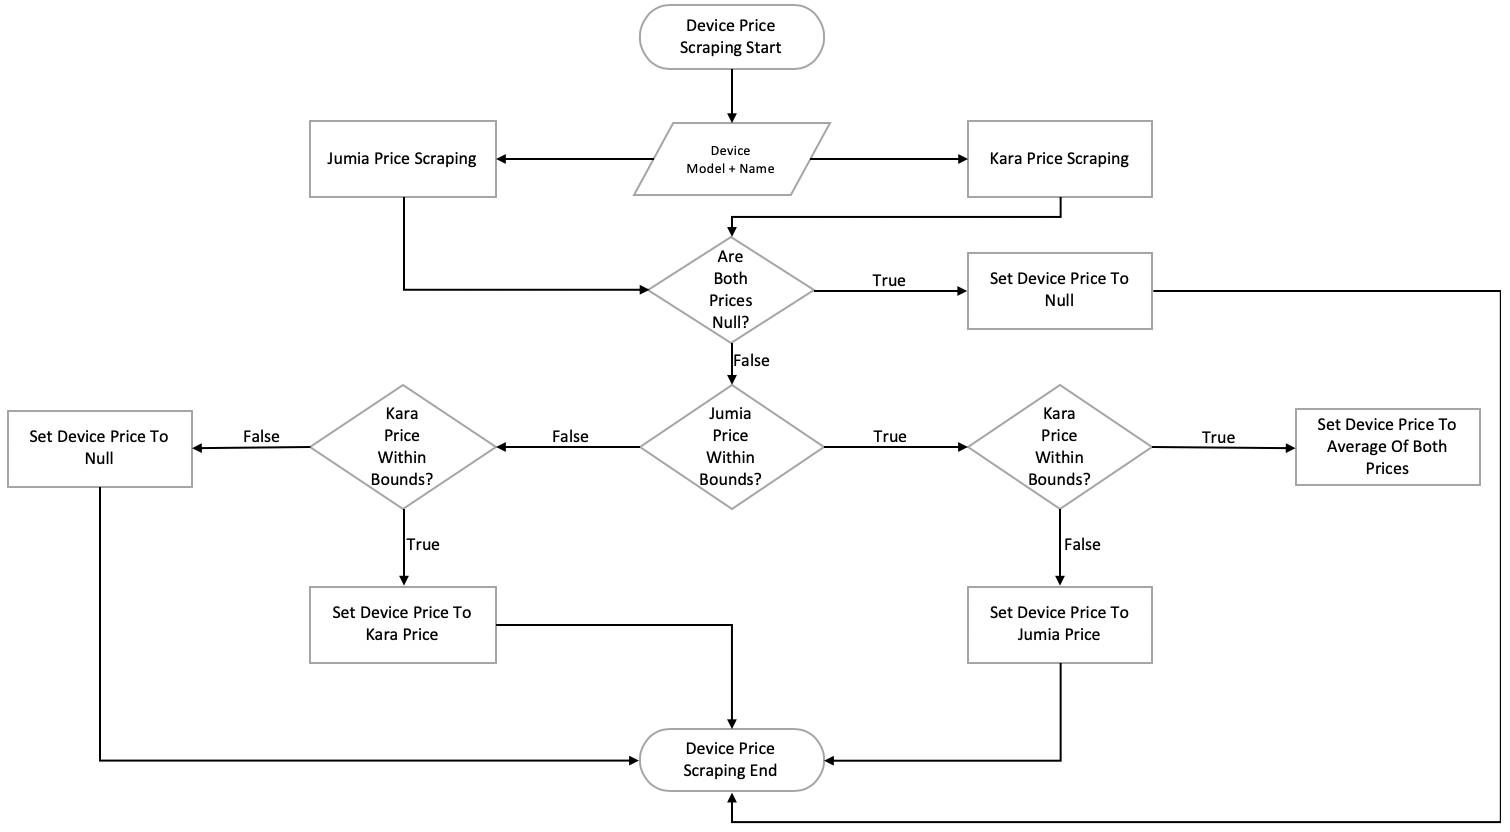
\includegraphics[width=0.9\textwidth]{images/device_price.png}
\caption{Device Price Logic}
\label{fig:device}
\end{figure}

\vspace{10pt}


Figure \ref{fig:device} displays the possible ways in which a device price could be determined. The possibilities are as follows: a price could not be scraped from either site, therefore, the price was set to null; a price could be scraped from one site but not the other, the scraped price was within the price bounds, then the one price was used; a price could be scraped from both sites, both prices were within the price bounds, then the price was set to be the mean of both prices. \\

Lower and upper price bounds were introduced to reduce the number of scraping miss-classifications and as a result improve data integrity. Unreasonably low prices were often device accessories such as phone cases or screen protectors. While unreasonably high prices were often laptops or other more expensive electronic devices.

%---------------------------------------------------------------------------------------
%	SECTION 3
%---------------------------------------------------------------------------------------

\section{Preprocessing}

\subsection{Missing Values}

Missing values are an issue that need to be addressed during any data science project, however missing data is especially significant in credit risk related modelling. Gathering complete credit repayment data is the most important factor when developing credit risk models \parencite{MissingValuesBos}.

\subsubsection{Target Variable}

Repayment data is often sparse and complex. Many consumers have missing values based on incompleteness but others have missing values based on the fact that credit term has not been reached. These challenges make it difficult to develop statistically significant datasets required for credit repayment prediction models \parencite{MissingValuesCR}. \\ 

The loan repayment data used in this minor dissertation was complete. Only loanees that had completed their entire loan tenor and that all all their instalments for that particular loan were used in the dataset. This ensured that the target variable, loan default, did not contain any missing values. 49,550 first time applicants with a complete loan cycle were collected, which was enough to develop statistically significant training and testing samples. 

\subsubsection{Predictor Variables}

Beyond repayment data, the features used to predict repayment often contain missing values and the fact that a particular feature is missing from a loan application can be indicative of default. \\

The observed data used to train the models developed throughout this project did contain missing values. In other data science projects, rows containing missing values are often removed from the dataset \parencite{MissingValues}.  In the case of this project excluding all cases containing a missing value was not feasible as too few sample would have remained to train and test a valid model. \\

Another common missing value imputation technique is to replace missing values with the mean (continuous variables) or mode (categorical variables) of their respective variable. This is a successful technique if the variables are considered to be missing at random. In the case of this project missing values were consider to be missing not at random.  \\


This is due to the fact that the loanees considered manually filled variables during their loan applications. loanees could have withheld or altered variables based on how they thought it would affect the outcome of their credit application \parencite{MissingValuesBos}.  


\subsection{Categorical Variables}

Min Max Scaler

\subsection{Class Balancing}

Smote 